%
% compile with pdflatex:
%   $ pdflatex homework-hw
% , yields homework-example.pdf
%    You might need to compile twice, if, e.g., you start using references
%

\documentclass[10pt,letterpaper,oneside]{article}
\usepackage[ascii]{inputenc}
\usepackage{graphicx}
\graphicspath{ {} }
\usepackage{amsmath,amsfonts,amssymb}
\usepackage[margin=1in]{geometry}
	\setlength{\parindent}{0em}
	\setlength{\parskip}{1em}



\newtheorem{theorem}{Theorem}

%%%% user definitions %%%%%%%%%%%%%%%%%%%%%%%

\newcommand{\Problem}[1]{\subsection*{Problem #1}}
\newcommand{\Part}[1]{\subsubsection*{Part #1}}
\newcommand{\Solution}{\subsubsection*{Solution}}

	% Forms for Big-Oh notation
\DeclareMathOperator{\Omicron}{O}
\DeclareMathOperator{\omicron}{o}

\newcommand{\BigOh}[1]{\Omicron(#1)}
\newcommand{\LittleOh}[1]{\omicron(#1)}
\newcommand{\BigOmega}[1]{\Omega(#1)}
\newcommand{\LittleOmega}[1]{\omega(#1)}
\newcommand{\BigTheta}[1]{\Theta(#1)}

	% Operators for dominance notation
\newcommand{\domeq}{\sim}
\newcommand{\domle}{\preceq}
\newcommand{\domlt}{\prec}
\newcommand{\domge}{\succeq}
\newcommand{\domgt}{\succ}

\newcommand\tab[1][1cm]{\hspace*{#1}}


%%%%%%%%  You edit stuff below this line  %%%%%%%%%%%%%%%%%%%%%%%%%%

\title{HW5 Theory}
\author{Alexander Kazantsev}
%\date{}  % uses today, by default

\begin{document}

\maketitle

\Problem{5.1}
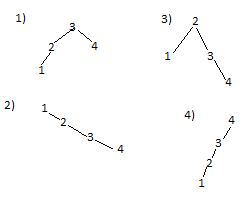
\includegraphics{5_1.png}

\Problem{5.2}
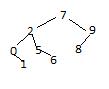
\includegraphics{5_2.png}
\Problem{5.3}
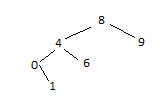
\includegraphics{5_3.png}

\Problem{5.4}
The order in which elements in a binary tree are deleted do no affect the final order of the binary tree.

\Problem{5}

n     \tab  T(n)

10     \tab  2.59876251221e-05

100   \tab   0.000167846679688

1000   \tab  0.00176882743835

10000  \tab  0.0182538032532

100000 \tab  0.186135053635

1000000 \tab 1.9062898159

Without the aide of a plot it is easily visible that $T(n)$ grows linearlly with the growth of $n$, $MH(n) \in \BigOh{n}$


\Problem{6}
It has been established that to build a heap it takes approxmiately linear time, which means it is bounded by $\BigOh{n}$

Next, the first and last element are swapped in the array and the size is decremented which is constant, $\BigOh{1}$

Finally, the first element is down heaped and the cycle continues from the second step. Each down heap costs $\BigOh{log(n)}$ and is repeated $n$ times, which yields a time complexity of $\BigOh{nlog(n)}$ using $Big Oh$ multiplicative rule. The size of the actual algorithm is constant as only two items are swapped at every iteration.


\Problem{7}

otherDS* holdOrder(otherDS data)

\tab if first(data) == NULL

\tab\tab return NULL

\tab otherDS *result = malloc( sizeof(otherDS) * len(data))

\tab result[0] = *first(data)

\tab count = 1

\tab while next(data) != NULL

\tab\tab result[count] = *next(data)

\tab\tab count += 1

\tab return result

end

double *copyHeight (otherDS data)

\tab if first(data) == NULL

\tab\tab return NULL

\tab float *result = malloc( sizeof(flaot) * len(data))

\tab result[0] = first(data)-$>$height

\tab count = 1

\tab while next(data) != NULL

\tab\tab result[count] = next(data)-$>$height

\tab\tab count += 1

\tab return result

end

void copyComputedValue( doubles d[], otherDS data)

\tab first(data)-$>$computed value = d[0]

\tab count = 1

\tab temp = next(data)

\tab while temp != NULL

\tab\tab temp-$>$computed value = d[count]

end

main()

\tab otherDS data = holdOrder( satelliteData )

\tab float *allHeight = copyHeight( data )

\tab copyComputedValue( impressiveA( allHeight ), data)


All of the functions written above operate at  $\BigOh{n}$ as they only iterate over $n$ elements. Since none of the operations are embedded the additivity rule can be used to determine the whole run time is at  $\BigOh{n}$. The space complexity is also  $\BigOh{n}$

\Problem{8}

.

.

struct SQ( // stack queue

\tab stack A

\tab stack B

)

Enqueue (SQ q, element x)

\tab push(q.A, x)

end

Remove(SQ q)

\tab while q.A not empty

\tab\tab push( q.B, pop( q.A ) )

\tab result = pop(q.B)

\tab while q.B not empty

\tab\tab push( q.A, pop( q.B ) )

\tab return result

end

The time complexity for insert in this implementation is constant, and the time complexity for remove is linear. The space complexity is $2n$ which simplifies to  $\BigOh{n}$

\Problem{9}

Math and all that jazz

I'm tired and I have to take the exam in 11 hours. So how about I tell you my favorite color. It's blue, becuase the sky is blue.

\end{document}